% !TEX root = main.tex
%%%%%%%%%%%%%%%%%%%%%%%%%%%%%%%%%%%%%%%%%%%%%%%%%%%%%%%%%%%%%%%%%%%%%%%%%%%%%%%%
% Survival Analysis
%%%%%%%%%%%%%%%%%%%%%%%%%%%%%%%%%%%%%%%%%%%%%%%%%%%%%%%%%%%%%%%%%%%%%%%%%%%%%%%%
\begin{figure*}
  \centering
  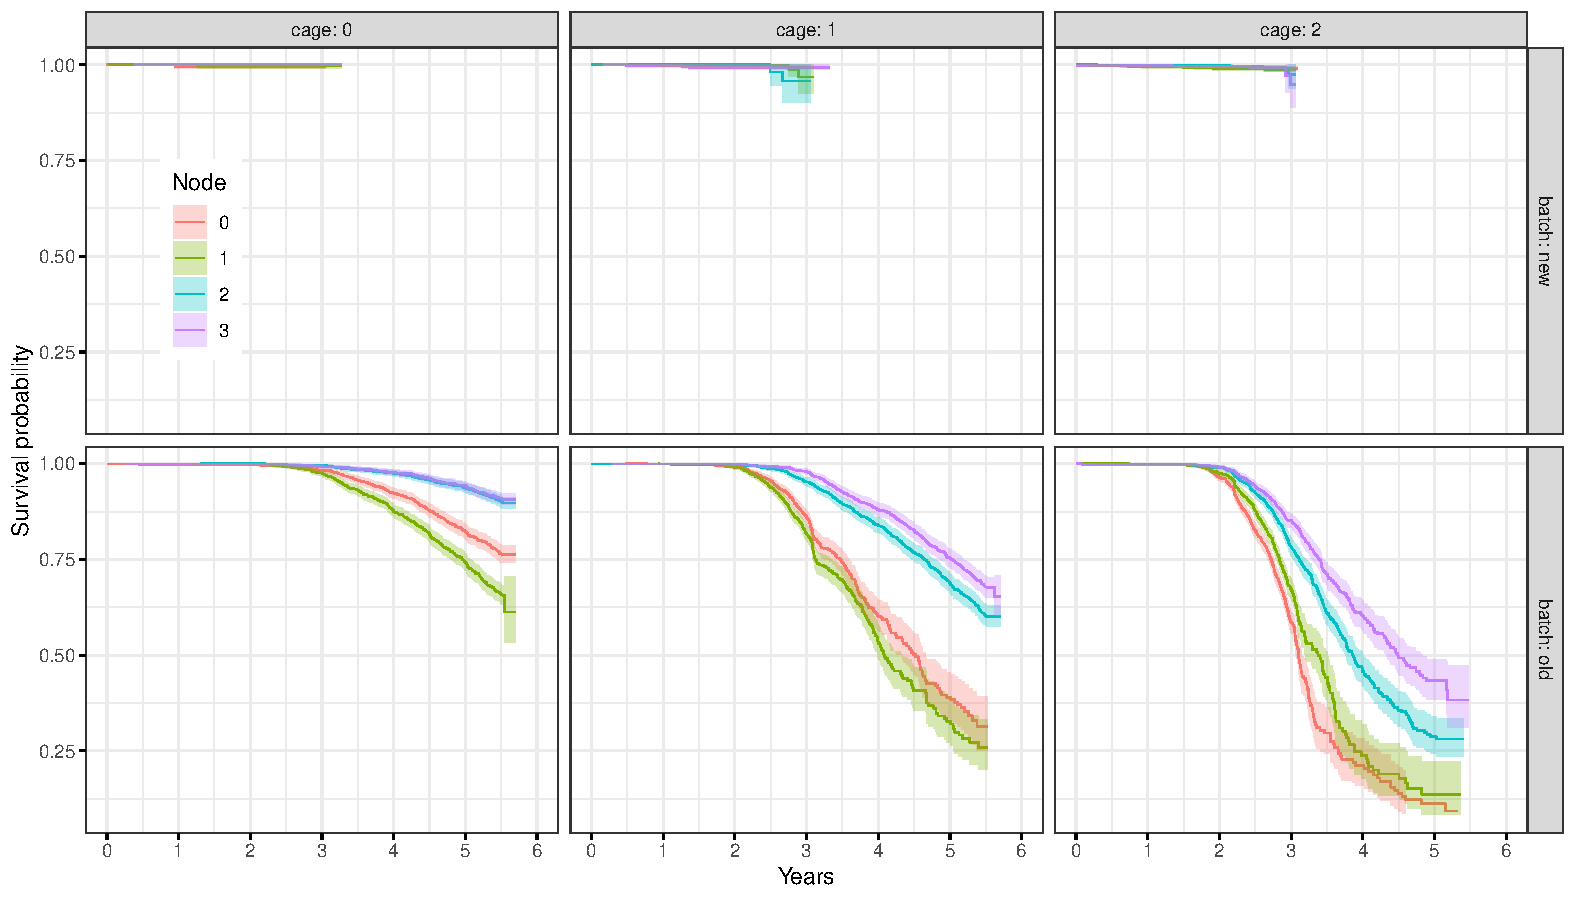
\includegraphics[width=7in]{figs/km_cage-node_a001.pdf}
  \caption{Comparison of the old and new batches, including survival
    differences based on {\tt cage} and {\tt node} GPU locations.}
  \label{fig:km-all-cage-node}
\end{figure*}
\section{Survival Analysis}
\label{section:survival}
\renewcommand{\pkg}[1]{\textsf{#1}}
Survival analysis (SA) methods, sometimes referred as time to event
methods, focus on the effect of the machine on the GPU units. This is
useful for determining factors that contribute to failures and
potentially for root cause analysis. SA methods use and combine
information across the operational lifetimes of all GPUs
\cite{survival}. For these analyses, we take apart the location string
of each GPU into variables {\em col, row, cage, slot, and node} and
study the influence of the locations on the GPU life times. The
construction of a GPU life time is more complex than it initially
appears because the units are observed only at reboot time, because
most units were proactively replaced to prevent failure, and because
some units continue in operation after OTB and DBE events (when a
second reboot may be successful).

A unit that experiences at least one OTB or DBE event and is removed
from the system is considered failed and its operation time until the
last seen time is taken as its life time. Although most failed units
experience one of these events at the last seen time, our definition
is not perfect because some units experience OTB or DBE events at a
time different from its last seen time. Such units were relatively few
so we consider this definition of life time as the most pragmatic.

A key concept in survival analysis is censoring, which is about using
information from study subjects whose exact failure times are not
available or that have not failed. This applies to our study because
of proactive GPU replacement before failure, because most units were
still in operation when the system was shut down, and also because
life spans were recorded only at inventory times. We use censoring
concepts on the proactive replacements and units still in operation at
the end. This allows us to use all of the GPU life time data,
including units that did not fail. But we ignore the inspection time
censoring, treating inventory times as exact failure times to reduce
the complexity of this analysis. We expect that because of the volume
of data and length of operation time, this would not make much
difference in our conclusions. However, we are making our data
publicly available and expect that others, especially in the survival
analysis community, will dive deeper.

Kaplan-Meier survival analysis (KM) starts with computing the
probability of survival beyond a given time. It is a nonparametric
technique that makes no specific failure model assumptions, such as
Weibull, Exponential, etc. The technique is able to use censored
observations and can also split the data into subpopulations to
compute separate survival curves.

If $T$ is the random variable of a GPU fail time, then its cumulative
distribution function $F(t) = Pr\{T < t\}$ gives the probability that
a GPU fails by duration $t$. The survival function is its complement
\begin{displaymath}
  S(t) = Pr\{T \geq t\} = 1 - F(t).
\end{displaymath}
It is the probability of being operational at duration $t$.  We use
the R packages \pkg{survival} and \pkg{survminer} for the KM analysis,
which is reported in Figure~\ref{fig:km-all-cage-node}. Within each
{\em batch}, separate survival curves are computed for each {\em cage}
by {\em node} combination. Along with the survival curve estimate,
this analysis provides 95\% confidence region for survival probability
shaded around the curves.
% Inserting figure here so it appears at top of next page
\begin{figure}
  \centering
  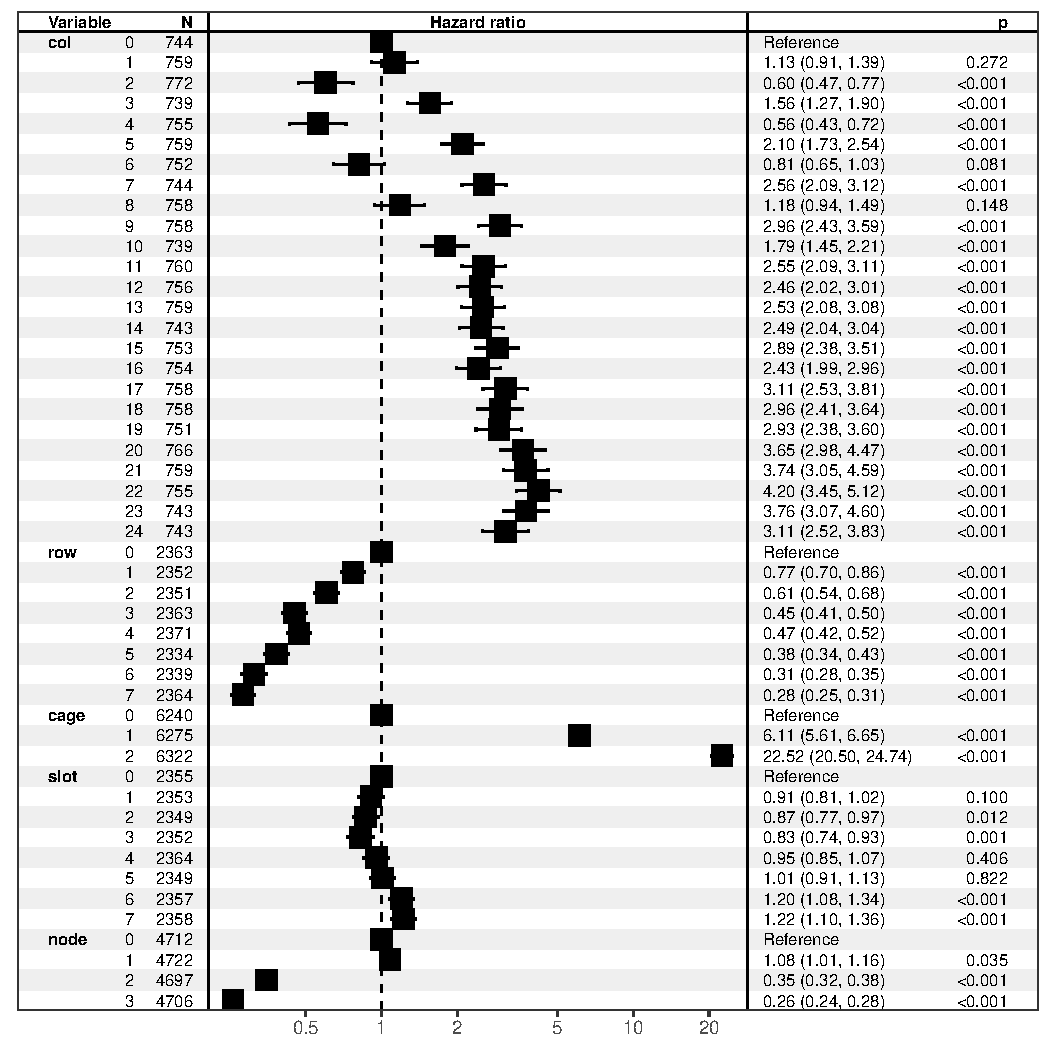
\includegraphics[width=\columnwidth]{figs/cox_o001.pdf}
  \caption{GPU hazard ratios from Cox regression model on {\tt old}
    batch.}
  \label{fig:cox-old}
\end{figure}
\begin{figure}
  \centering
  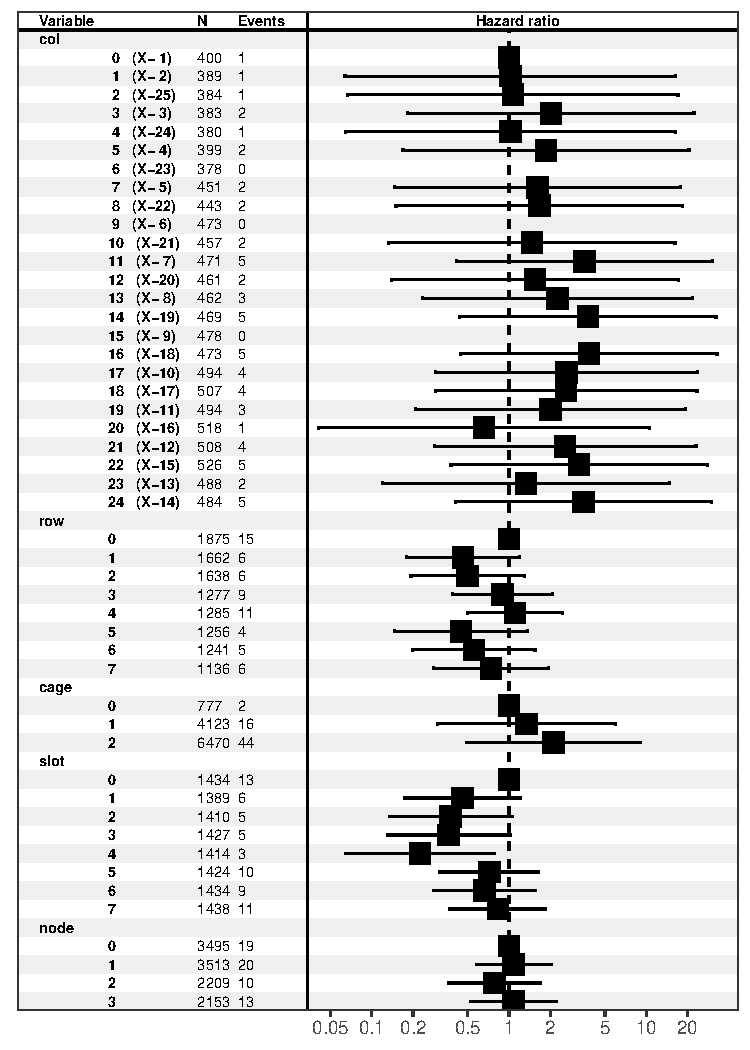
\includegraphics[width=\columnwidth]{figs/cox_n001.pdf}
  \caption{GPU hazard ratios from Cox regression model on {\tt new}
    batch.}
  \label{fig:cox-new}
\end{figure}

It appears that transport of cooling air provides a complete
explanation for relative differences in cage and node survival rates
in the old batch.  We reach this conclusion with reference to
Figure~\ref{fig:layout} and relative positions of cages and nodes
within a cabinet. Both cage and node differences in survival
probabilities can be explained by an inverse relationship with the
distance to the bottom of the cabinet, where cooling air is forced
through the cabinet to the top. The survival curves can be ordered
({\em cage 0, cage 1, cage 2}) in decreasing order of survival. As the
blades are placed vertically within the cabinet, pairs of nodes too
experience the same relationship with distance to the bottom, nodes 2
and 3 having lower failure rates than nodes 0 and 1.

Very few failures have occurred in the new batch and they are clearly
less prone to failure at the 2.5 year mark. There is a slight change
at the 3 year mark of cages 1 and 2 but it is also accompanied with a
rise in uncertainty and survival is still well above levels in the old
batch.

We don't see a ``bathtub curve'' phenomenon, in fact the opposite is
apparent in cages 1 and 2 of the old batch. The slope of the survival
curve is related to the hazard rate. There does not seem to be an
early ``infant mortality'' period nor a ``wearout'' phenomenon at the
end. Rather, we see a steeper slope (higher hazard rate) in the
middle, associated with the unexpected resistor failures.

To get more comparison power across the locations, we can use a
technique that in a sense averages over time. Cox proportional hazards
(CPH) regression analysis, can include covariates and estimates relative
risk averaged over time based on the covariates
\cite{Cox1972,Harrell2015}. The CPH regression function takes the form
\begin{displaymath}
  h(t) = h_0(t)e^{b_1 x_1 + b_2 x_2 \ldots b_k x_k},
\end{displaymath}
where $x_i$ are covariates, $h_0(t)$ is the {\em baseline hazard}, and
the $b_i$ are coefficients that measure the impact of the
covariates. The quantity $e^{b_i}$ is the hazard ratio (increased
average risk over baseline) for covariate $i$.

CPH is considered a semi-parametric model as there are no assumptions
about the shape of the baseline hazard function. Its strongest
assumption is that the hazards are proportional. There are a number of
tests for this, including graphical diagnostics in the \pkg{survminer}
package as well as checking that survival curves for categorical
covariates do not cross. We ran these diagnostics and concluded that
the hazards for our location categories are approximately
proportional. However, survival functions partitioned on {\em batch}
do cross and so we fit the model to the new and the old batches
separately. The results are presented in Figures~\ref{fig:cox-old}
and~\ref{fig:cox-new}.

We find that the average hazard ratios strongly correlate with
detailed nuances of the system cooling architecture.  The figures give
hazard ratios for each of the location variables, giving the ratio for
each level compared to its first (0) level (consequently the 0 level
is always 1). Due to the exponential nature of the CPH model, the
horizontal hazard ratio axis is on a log scale. The estimates include
uncertainty, which too is most reliably computed on a log scale (see,
for example, \cite{Ostrouchov88}). In the figures, we also include the
number of units, N, at risk and the number of events that occurred in
each category.

All the factors ({\em col, row, cage, slot, node}) in the old batch
are balanced with respect to the number of units at risk and
consequently nearly orthogonal (each level of a factor contains all
levels of the other factors) seemingly an almost ``designed''
experiment nature to this analysis. This is not the case for the new
batch, where the cage levels have very different numbers of units at
risk. But this also points out that even for the old batch the balance
holds only at the outset and as life proceeds, failing units are
replaced with new units and the balance degrades because failures are
location-dependent.

Our interpretation of correlation with details of the cooling system
comes mostly from the hazard ratios for the old batch. The new batch
has mot had many failure events and the uncertainty bars of nearly all
ratios include 1, which is no difference. In the old batch, we see
that {\em cage} has the strongest effect, putting the highest hazard
ratio on cage 2, which is consistent with lowest survivals in the KM
analysis earlier. Its ratio value near 20 has to be interpreted with
caution because it is a time averaged value on a log scale and suffers
from the degrading balance mentioned in the previous paragraph. This
aspect is not captured by the uncertainty, which accounts for the
randomness of the failures and not for the geometric time averaging
\cite{coxhazardinterpret}. Consequently, we interpret the pattern of
relative hazards rather than actual ratio magnitudes. More in-depth
analysis with penalized estimation methods like \cite{bender2019} can
take such balance issues in the exposure history into account and
provide time-dependent hazard estimates.

In addition to the strong {\em cage} and {\em node} hazard rate
differences that increase with distance from the bottom of the
cabines, seen in both KM and CPH results, there is a weaker but
peculiar pattern in the {\em row} and {\em col} hazard rates. The
different behavior in {\em col} 0-11 from {\em col} 12-24 is likely
due to separate supply lines of chilled water to the two sets. While
the temperature was a consistent 42$^\circ$F, there may have been
minor flow or pressure differences. But the interleaving pattern of
the first set is still a mystery. We also have yet to explain the
apparent row effects. A very minor airflow effect across slots also
seems to be present as it mimics faster airflow for the middle slots.
